\documentclass[notes]{subfiles}
\begin{document}
	\chapter{Ingredients of Change: Functions \& Limits}
	\addcontentsline{toc}{section}{1.1 - Functions: Four Representations}
	\setcounter{section}{1}
	\setcounter{page}{1}
	\fancyhead[RO,LE]{\bfseries \large \nameref{cs11}} 
	\fancyhead[LO,RE]{\bfseries \currentname}
	\fancyfoot[C]{{}}
	\fancyfoot[RO,LE]{\large \thepage}	%Footer on Right \thepage is pagenumber
	\fancyfoot[LO,RE]{\large Chapter 1.1}
	

	
\section*{Functions: Four Representations}\label{cs11}
	\subsection*{Representations of Change}
		In mathematics, particularly applied mathematics, we need to be able to interpret real-world phenomena in four ways: numerically, algebraically, verbally, and graphically.  

		\begin{ex}
			The price of gas at a certain 7-11 in Norman was \$4.39 per gallon on June 26th.  Represent this data in four ways.
		\end{ex}
		
			\begin{enumerate}[(1)]
				\item \emph{Numerically}: We can numerically represent the data by placing values in a table.
					\begin{center}
						{\renewcommand{\arraystretch}{1.2}
						\begin{tabular}{|c||c|c|c|c|c|c|}\hline
							\textbf{Gasoline Pumped} (in gallons) & 0 & 1 & 5 & 10 & 15 & 20 \\ \hline
							\textbf{Total Cost} (in USD) & 0 & 4.39 & 21.95 & 43.90 & 65.85 & 87.80\\ \hline
						\end{tabular}
						}
					\end{center}
						%Do i want to actually make them fill this out?
						 
				\item \emph{Algebraically}: 
					Since we are paying \$4.39 for every gallon, it is reasonable to express the situation by the function $p(g) = 4.39g$ dollars (total cost), with $g$ gallons pumped.
										
				\item \emph{Verbally}: 
					The problem is given to us verbally, but using we'll rephrase it to sound more like what we would expect in this class.  The price at the pump for gasoline is \$4.39 per gallon of gasoline pumped.
				
				\item \emph{Graphically}: 
					We may use a graph to display this same information.  Since we created the function $p(g) = 4.39g$, we can plot this in order to create a graphical representation of the data.  
					\begin{center}
						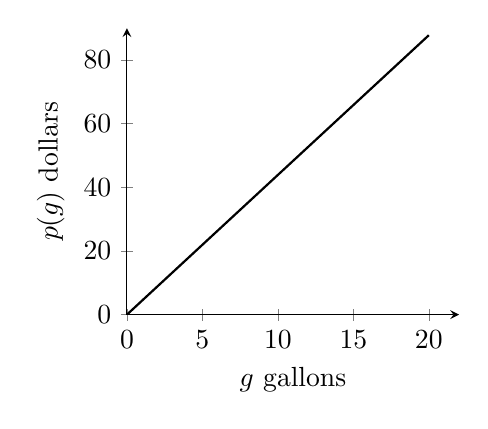
\begin{tikzpicture}
							\begin{axis}
								[
									axis x line = bottom,
									axis y line = left,
									xlabel = {$g$ gallons},
									ylabel = {$p(g)$ dollars},
									scale only axis=true,
									height = .3\textwidth,
									xmax = 22,
									ymax = 90
								]
								\addplot[thick, domain = 0:20] {4.39*x};
							\end{axis}
						\end{tikzpicture}
					\end{center}
			\end{enumerate}
	
		\noindent The process of using information like this to generate something usable is called \emph{mathematical modeling}, and we call the result a \textbf{model}.  Business Calculus courses place heavy emphasis on developing and deploying models. 
		 
	\subsection*{Functions \& Representations}
		A \textbf{relation} is a rule which links an \textbf{input} variable to an \textbf{output}; given one piece of information, we can determine the corresponding piece.  A special type of relation is one called a function.
		
		\begin{defn}[Function]
			A \textbf{function} is a rule that assigns \fitb{a single output per input value}{\makebox[3in]{\hrulefill}}.  For a given output function $f$, and given input value $x$, this is notated $f(x)$.  
		\end{defn}
		
		\noindent \textsc{it is very important that you understand this notation}.  One of the most common mistakes in 1743 and 2123 is a misunderstanding of how function notation works.  The letters chosen ($f,g,h,k,g,A,$ etc.) indicate the \emph{name} of the function, and the numbers/variables inside the parentheses indicate \emph{what the function is being applied to}.  A way to remember this is to read the expression $f(x)$ as ``$f$ of $x$''.
			\newpage
			
		\begin{ex}
			Let $g$ be a function.  Write the correct notation for the following situations:
				\begin{enumerate}[(a)]
					\item $g$ applied to the number 5
						\vs{1}
					\item $g$ applied to the number 10
						\vs{1}
					\item $g$ applied to the variable $x$
						\vs{1}
					\item $g$ applied to the variable $y$
						\vs{1}
					\item $g$ applied to the expression $x + 1$
						\vs{1}
					\item $g$ applied to the expression $10 - y$
						\vs{1}
					\item $g$ applied to the expression $x + h$
						\vs{1}
				\end{enumerate}
		\end{ex}
			\newpage
		\begin{ex}
			Evaluate the function $f(x) = 3x - 2$ at the inputs:
			\begin{enumerate}[(a)]
				\item $x =2$
					\vs{1}
				\item $x = 3$
					\vs{1}
				\item $x = -4$
						\vs{1}
				\item $x = k$
						\vs{1}
				\item $x = k+7$
						\vs{1}
				\item $x = 3k + 21$
						\vs{1}
				\end{enumerate}
		\end{ex}
		\noindent We may also represent functions using an \textbf{input/output diagram}.  One is given below, for the previous example:
			\begin{center}
				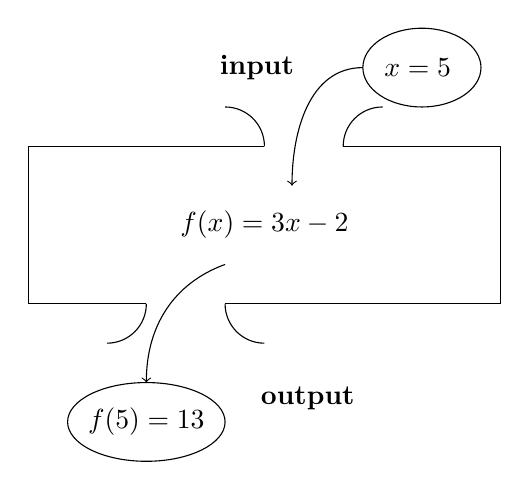
\begin{tikzpicture}
					\draw (-1.5,-1)--(-3,-1)--(-3,1)--(0,1); %left piece of diagram
					\draw (1,1)--(3,1)--(3,-1)--(-.5,-1); %right piece of diagram
					\draw (-.5,1.5) to [out = 0, in = 90] (0,1); %left piece of input pipe
					\draw (1.5,1.5) to [out = 180, in = 90] (1,1); %right piece of input pipe
					\draw (-2,-1.5) to [out = 0, in = 270] (-1.5,-1); %left piece of output pipe
					\draw (0,-1.5) to [out = 180, in = 270] (-.5,-1); %right piece of output pipe
					\draw[->] (1.25,2) to [out = 180, in = 90] (.35,.5); %input arrow
					\draw (1.4,2) node[right] {$x =5$}; %input value
					\draw (2,2) ellipse (.75cm and .5cm); %ellipse for input
					\draw (0,0) node {$f(x) = 3x-2$}; %function
					\draw[->] (-.5,-.5) to [out = 200, in = 90] (-1.5,-2); %output arrow
					\draw (-1.5,-2.5) ellipse (1cm and .5cm); %output ellipse
					\draw (-1.5,-2.5) node {$f(5) = 13$}; %output value
					\draw (.5,2) node[left] {\textbf{input}}; %input label
					\draw (.55,-2.2) node {\textbf{output}}; %output label
				\end{tikzpicture}
			\end{center}
			\newpage
			
		\noindent Every function is a relation, but not every relation is a function.  If a relation gives more than one output value for even a single input value, then it cannot be a function.  This can be determined using a verbal, numerical, or graphical description of the data.
	\begin{ex}
		Let $C(t)$ represent the number courses offered campus-wide during the week at time $t$, and $O(t)$ represent the number of students walking on the South Oval at time $t$ last Monday.   Is $C$ a function?  What about $O$?
		\end{ex}	
			\vs{1}
		\begin{ex} 
			Below are numerical expressions for the functions $h$ and $k$.  Is $h$ a function?  What about $k$?
			\begin{center}
				{\renewcommand{\arraystretch}{1.2}
				\begin{tabular}{|c|c|c|c|c|c|c|} \hline
					$x$ & 0 & 1 & 1 & 2 & 5 & 6 \\ \hline
					$h(x)$ & 0& 1 & 2 & 3 & 4 & 5 \\ \hline
				\end{tabular}\hspace*{15pt}
				\begin{tabular}{|c|c|c|c|c|c|c|} \hline
						$t$ & 0 & 1 & 1 & 2 & 5 & 6 \\ \hline
						$k(t)$ & 0 & 1 & 1 & 3 & 4 & 5 \\ \hline
					\end{tabular}
				}
				\end{center}
		\end{ex}			
			\vs{1}

		\begin{ex}
			Are both of these graphs functions?  Why or why not?
			\begin{center}
				\begin{tabular}{lr}
					\begin{tikzpicture}
						\begin{axis}[
							axis x line = middle,
    						axis y line = middle,
	    					every axis y label/.style=
{at={(ticklabel cs:1.1)}},
							y label style={at={(axis description cs:0,1.1)},anchor=north},
	    					ylabel = {$y$},
    						every axis x label/.style= {at ={(ticklabel cs:1)}},
    						x label style={at={(axis description cs:1.1,.48)},anchor=east},
    						xlabel = {$x$},
							trig format plots = rad,
							xmin = 0, xmax = 6.5,
							ymin = -1.5, ymax = 1.5
						]
						\addplot[thick, smooth, domain = 0:2*pi] {cos(x)};
						\end{axis}
					\end{tikzpicture}
				&
					\begin{tikzpicture}
	  	  				\begin{axis}[
    						axis x line = middle,
    						axis y line = middle,
	    					every axis y label/.style=
{at={(ticklabel cs:1.1)}},
							y label style={at={(axis description cs:.5,1.1)},anchor=north},
	    					ylabel = {$y$},
    						every axis x label/.style= {at ={(ticklabel cs:1)}},
    						x label style={at={(axis description cs:1.1,.65)},anchor=east},
    						xlabel = {$x$},
							xmin=-4.5,xmax=4.5,
       			    		ymin=-9.5,ymax=4.5,
			       		    xtick = {-4,-2,2,4},
	    		   		    ytick = {-8,-6,-4,-2,2,4},
        		    	]
        			    \addplot [domain=-3:3,samples=50]({x^3-3*x},{3*x^2-9}); 
	   				 \end{axis}
					\end{tikzpicture}
				\end{tabular}
			\end{center}
		\end{ex}
		\vs{1}
		\newpage

	\subsection*{Model Output and Units of Measure}
		In real-world applications, the proper units of measure must be attached to a model and every result derived from that model; in this way, we can gain meaningful information from whatever is it we do.  The verbal description of a function gives us the units of measure.  In our first example, our input unit is \emph{gallons}, and our output unit is \emph{dollars}. 

		
		\begin{ex}
			The population of Canada between 1900 and 2010 is given by the model
				\[p(t) = 3(1.03^t)\text{ million people}\]
			where $t$ is the number of years since the end of 1900.
			\begin{enumerate}[(a)]
				\item When did the population reach 155 million people?  Write a sentence interpreting the result.
					\vs{1}
				\item Determine the population in the year 1990.  Write a sentence interpreting the result.
					\vs{1}
				\item Give a description and the unit of measure for both the input and output variables.
					\vs{1}
				\item Draw an input/output diagram for $p$, and a graph of $p$.
					\vs{1}
			\end{enumerate}
		\end{ex}
			\newpage

		\begin{ex}
			Calculate the output value that corresponds to the inputs $t = 4.5$ and $t = -2$ for the function $m(t) = \dfrac{3}{8}t + 2$.
		\end{ex}
			\vs{1}

		\begin{ex}
			Calculate the output value that corresponds to the inputs $x = 10$ and $x = -3$ for the function $f(x) = 7x^2 -2x-3$.
		\end{ex}
			\vs{1}
		\begin{ex}
			Let $f(x) = 2.5\ln x + 3$.
			\begin{enumerate}[(a)]
				\item Does the expression $f(x) = 7$ ask to find an input or output?
					\vs{.5}
				\item Solve (a).
					\vs{1}
			\end{enumerate}
		\end{ex}
			\newpage

		\begin{ex}
			Let $f(x) = 6.1x + 3.1^x$.
			\begin{enumerate}[(a)]
				\item Does the expression $x = 2.5$ ask to find an input or output?
					\vs{.5}
				\item Solve (a).
					\vs{1}
			\end{enumerate}
		\end{ex}
			
		\begin{ex}
			Let $u(t) = \dfrac{27.4}{1+13e^{2t}}$.
			\begin{enumerate}[(a)]
				\item Does the expression $u(t) = 15$ ask to find an input or output?
					\vs{.5}
				\item Solve (a).
					\vs{1}
			\end{enumerate}
		\end{ex}
		

		\begin{ex}
			The number of donors to the American Red Cross Disaster Relief Fund who donated more than $x$ million dollars during 2005 is represented as $d(x)$.
			\begin{enumerate}[(a)]
				\item Write a sentence of interpretation for $d(5) = 2$.
					\vs{1}
				\item Write the function notation for the statement: ``Seventy-five groups donated at least \$500,000 to the Disaster Relief Fund in 2005.'' 	
					\vs{.5}
			\end{enumerate}
		\end{ex}
		
		\begin{ex}
			The average number of people standing in the Chick-Fil-A line on Wednesdays can be represented by $p(t)$, where $t$ is the number of hours after 12:00pm.
			\begin{enumerate}[(a)]
				\item Write a sentence of interpretation for the expression $p(0) = 32$
					\vs{1}
				\item Write the function notation for the statement ``At 1:15pm, there are an average of 15 people in line at Chick-Fil-A''.
					\vs{.5}
			\end{enumerate}
		\end{ex}
		\clearpage
\end{document}